% Autor šablony: Jakub Dokulil (kubadokulil99@gmail.com) https://github.com/Kubiczek36/SOC_sablona

\documentclass[12pt, a4paper,
  oneside,      %% -- odkomentujte, pokud chcete svou práci mít pouze jednostrannou, mezera pro hřbet pak automaticky bude pouze na levé straně
 %% twoside,        %% -- pro oboustranné práce, mezera pro hřbet následně střídá strany.
 %% openright
]{report}

%% Nutné balíčky a nastavení
%%%%%%%%%%%%%%%%%%%%%%%%%%%%

\newcommand\city{Pardubice} 
\newcommand\district{Pardubický}
\newcommand\specialization{Obor č. 18: Informatika}
\newcommand\school{SŠIE Delta}
\newcommand\consultant{RNDr. Koupil Jan, Ph.D.}
\newcommand\name{Krátký Kryštof}
\newcommand\public% Autor šablony: Jakub Dokulil (kubadokulil99@gmail.com) https://github.com/Kubiczek36/SOC_sablona

\title{Histories} %% -- Název tvé práce
\author{\name} %% -- tvé jméno
\date{\publicationYear} %% -- rok, kdy píšeš SOČku

\usepackage[top=2.5cm, bottom=2.5cm, left=2cm, right=2cm]{geometry} %% nastaví okraje, left -- vnitřní okraj, right -- vnější okraj

\usepackage[czech]{babel} %% balík babel pro sazbu v češtině
\usepackage[utf8]{inputenc} %% balíky pro kódování textu m
\usepackage[T1]{fontenc}
\usepackage{cmap} %% balíček zajišťující, že vytvořené PDF bude prohledávatelné a kopírovatelné

\usepackage{graphicx} %% balík pro vkládání obrázků

\usepackage{subcaption} %% balíček pro vkládání podobrázků

\usepackage{hyperref} %% balíček, který v PDF vytváří odkazy

\linespread{1.15} %% řádkování

\usepackage[pagestyles]{titlesec} %% balíček pro úpravu stylu kapitol a sekcí
\titleformat{\chapter}[block]{\scshape\bfseries\LARGE}{\thechapter}{10pt}{\vspace{0pt}}[\vspace{-22pt}]
\titleformat{\section}[block]{\scshape\bfseries\Large}{\thesection}{10pt}{\vspace{0pt}}
\titleformat{\subsection}[block]{\bfseries\large}{\thesubsection}{10pt}{\vspace{0pt}}

\setcounter{secnumdepth}{2}
\setcounter{tocdepth}{1}
\usepackage{fancyhdr}
\pagestyle{fancy}
\renewcommand{\headrulewidth}{1pt}

\newenvironment{propertiesItemize}{
\begin{itemize}{ 
  }}
  {\end{itemize}}

\usepackage{booktabs}

\usepackage{url}

%% Balíčky co se můžou hodit :) 
%%%%%%%%%%%%%%%%%%%%%%%%%%%%%%%

\usepackage{pdfpages} %% Balíček umožňující vkládat stránky z PDF souborů, 

\usepackage{upgreek} %% Balíček pro sazbu stojatých řeckých písmen, třeba u jednotky mikrometr. Například stojaté mí: \upmu, stojaté pí: \uppi

\usepackage{amsmath}    %% Balíčky amsmath a amsfonts 
\usepackage{amsfonts}   %% pro sazbu matematických symbolů
\usepackage{esint}     %% pro sazbu různých integrálů (např \oiint)
\usepackage{mathrsfs}

%% makra pro sazbu matematiky
\newcommand{\dif}{\mathrm{d}} %% makro pro sazbu diferenciálu, místo toho
%% abych musel psát '\mathrm{d}' mi stačí napsat '\dif' což je mnohem 
%% kratší a mohu si tak usnadnit práci

%% Bordel pro práci - můžeš smáznout :) 
%%%%%%%%%%%%%%%%%%%

\usepackage{lipsum} %% balíček který píše lipsum (nesmyslný text, který se používá pro kontrolu typografie)

%% Začátek dokumentu
%%%%%%%%%%%%%%%%%%%%


\begin{document}

\pagestyle{empty}
\pagenumbering{Roman}

\begin{titlepage}
    \bfseries{ %%% písmo na stránce je tučně
        \begin{center}
            \LARGE{STŘEDOŠKOLSKÁ ODBORNÁ ČINNOST} 
            \vspace{14pt}
            \large{\specialization} 

            \vspace{0.4 \textheight}

            \LARGE{ %%%%
                Histories
            }%%%%

            \vspace{0.4\textheight}
        \end{center}
        
        \noindent\Large{\name}

        \noindent\Large{\district\hspace{\stretch{1}}  \city, \publicationYear} %% vyplň oficiální název kraje, město a rok
        
            
    } %%%
\end{titlepage}

\cleardoublepage%% Úvodní stránka s informacemi
{\bfseries %%% písmo na stránce je tučně
    \begin{center}
        \LARGE{STŘEDOŠKOLSKÁ ODBORNÁ ČINNOST}

        \vspace{14pt}
        {\large \specialization}

        \vspace{0.3 \textheight}

        \LARGE{ %%%%
        Histories
        }

        \LARGE{ %%%%
        platforma pro sdílení historických fotek
        }%%%%

        \vspace{0.24\textheight}
    \end{center}  
}%%%
{\Large %%%
    \noindent\textbf{Jméno:} \name\\
    \textbf{Škola:} \school\\
    \textbf{Kraj:} \district\\
    \textbf{Konzultant:} \consultant\\
} %%%

\noindent \city, \publicationYear\cleardoublepage\noindent{\Large{\bfseries{Prohlášení}}}  %% uprav si koncovky podle toho na jaký rod se cítíš, vypadá to pak lépe :) 

\noindent Prohlašuji, že jsem svou práci SOČ vypracoval/a samostatně a použil/a jsem pouze prameny a literaturu uvedené v seznamu bibliografických záznamů.

\noindent Prohlašuji, že tištěná verze a elektronická verze soutěžní práce SOČ jsou shodné. 

\noindent Nemám závažný důvod proti zpřístupňování této práce v souladu se zákonem č. 121/2000 Sb., o právu autorském, o právech souvisejících s právem autorským a o změně některých zákonů (autorský zákon) ve znění pozdějších předpisů. 

\vspace{24 pt}

\noindent V Pardubicích dne 9.\ září 2022 \dotfill{}\hspace{\stretch{0.5}} 

\hspace{8cm} \name\cleardoublepage\vspace*{0.8\textheight}
\noindent{\Large{\bfseries{Poděkování}}}

\noindent
Rád bych poděkoval svému konzultantovi RNDr. Janu Koupilovi, Ph.D. za odborné vedení a konzultace při tvorbě tohoto projekt.

\cleardoublepage\noindent{\Large{\bfseries{Abstrakt}}}

\noindent TBD abstrakt

\vspace{18pt}

\noindent{\Large{\bfseries{Klíčová slova}}}

\noindent Webová aplikace; sociální síť; sdílení historických fotek

\vspace{18pt}

\noindent{\Large{\bfseries{Abstract}}}

\noindent TBD abstract

\vspace{18pt}

\noindent{\Large{\bfseries{Keywords}}}

\noindent Web app; social media; historical photo sharing

\cleardoublepage\tableofcontents

\pagenumbering{arabic}
\pagestyle{fancy}
\setcounter{page}{1}


\chapter{Pojmy}
\subsection{NSFW}
Zkratka vycházející z~anglického \uv{Not Safe For Work} (nevhodné pro práci), zpravidla se takto označují příspěvky obsahující nahotu, nebo násilí, a tudíž by se jim mělo vyhnout v~profesionálním prostředí. \cite{NSFW}

\subsection{Garbage collection} Garbage collector se stará se o~uvolnění úseků v~paměti, které nejsou žádným procesem využívány \cite{GarbageCollection}

\subsection{Runtime environment} Jedná se o skupinu software umožňující spuštění programu v~reálném čase, obvykle implementuje základních funkce jako je například výpis textu nebo připojení k~internetu \cite{whatIsRuntimeEnvironment}


\chapter{Úvod}
Všichni ví, jak vypadá těch pár míst, se kterými se každodenně setkávají. Málo kdo ale tuší, jakou zajímavou mají daná místa historii, jak vypadala před 20, nebo 100 lety. Existují online komunity, které si přesně toto uvědomují. Bohužel jsou tyto komunity nucené využívat standardní platformy, které nemají fungovat jako archiv, ale naopak počítají pouze s prohlížením nově nahraného obsahu. To činí prohledávání, nebo řazení fotografií téměř nemožným. Cílem tohoto projektu bylo vytvořit platformu, která bude na míru šitá potřebám zmíněných komunit a umožní komukoliv snadné prohlížení historických fotografií. Mezi hlavní funkce patří zobrazování míst na mapě, komunikace s ostatními uživateli pomocí komentářů a možnost filtrování a řazení fotografií podle data jejich vzniku. 

 
\section{Existující řešení}
\subsection{Historypin}
Historypin je open-source platforma fungující jako archiv historických fotografií. Umožňuje vyhledávání míst na mapě, filtrování příspěvků podle data pořízení fotografie, nebo např. vytváření kolekcí. Obsahuje velké množství příspěvků, což kvůli špatně optimalizaci stránky vede k~pomalému načítání dat a nepřehlednosti mapy. Celá platforma je v angličtině a česká komunita na ní téměř neexistuje.

\subsection{Facebook}
Facebook je jedna z nejznámějších sociálních sítí zaměřující se na komunikaci uživatelů. Uživatelům umožňuje vytváření skupin (komunit), nebo například přidávání příspěvků. Primárním účelem Facebooku zůstává sdílení co nejaktuálnějšího obsahu. Neposkytuje téměř žádné možnosti filtrování příspěvků, či propojení s mapou. Ačkoliv zde jsou komunity  jako je například \uv{Pardubice v běhu času}, nebo \uv{Historické Karlovy Vary ve fotografii}.

%% POUŽITÉ TECHNOLOGIE
\chapter{Použité technologie}
V~projektu byly použity moderní a v~současné době jedny z nejpoužívanějších technologií pro zajištění co nejdelší podpory aplikace.
%% TECHNOLOGIE NA FRONTENDU I BACKENDU
\section{Technologie použité na frontendu i na backendu}
    %% TYPESCRIPT
    \subsection{Typescript}
    Typescript je nadstavba na JavaScript, umožňující statické typování \cite{DynamicVsStaticTyping}. Veškerý kód napsaný v~JavaScriptu je validním také v~Typescriptu. \cite{whatIsTypescript}\cite{typescriptForTheNewProgrammer}

    %% NPM
    \subsection{NPM}
    NPM je největším registrem JavaScriptových balíčků (knihoven) tvořených komunitou. Umožňuje jednoduchou instalaci balíčků pomocí CLI (command line interface). Konfigurační soubor obsahuje seznam všech balíčků použitých v~projektu včetně jejich verzí, což zamezuje chybám v~kódu z~důvodu změn v~nových verzích balíčků. \cite{whatIsNpmW3}\cite{aboutNpm}

    %% GRAPHQL
    \subsection{GraphQL}
    GraphQL je dotazovací jazyk pro API \cite{graphqlIntroduction}. Nejpoužívanější alternativou pro GraphQL je REST. Oproti REST u~GraphQL klient v~requestu specifikuje požadovaná data, která jsou následně vrácena serverem. Tím je eliminován přenos nepotřebných, nebo duplicitních dat, čímž je celá operace urychlena. GraphQL je silně typované \cite{graphqlTypes}, což znamená že musí být předem stanovený typ vrácených dat. \cite{restApiRedHat}\cite{whatIsApiAws}


%% FRONTEND 
\section{Technologie pro frontend}
Část webové aplikace, se kterou uživatel přímo interaguje (klientská strana) je označována za frontend aplikace. Obsahuje všechny prvky, se kterými se uživatel dostává do kontaktu přímo (např. texty, obrázky, tlačítka atd.). Frontend uživateli umožňuje ovládat aplikaci bez znalosti programování, nebo hlubší znalosti technologií, na kterých je postavena. Za frontend lze označit také mobilní, nebo desktopové aplikace. \cite{whatIsFrontend}

    %% REACT 
    \clearpage
    \subsection{React}
    React je open-source JavaScriptová knihovna (občas bývá označován za framework) využívaná na frontendu a pro tvorbu uživatelských rozhraní složených z~komponent viz \ref{subsubsection:reactComponents}. Komponenty jsou části kódu, které lze znovu používat čímž se předchází duplicitnímu kódu. Mezi hlavní funkce Reactu patří také state management a následné vykreslování DOMu (document object model). DOM je objektově orientovaná reprezentace webové stránky usnadňující její modifikaci. \cite{reactComponentsAndProps}\cite{gettingStartedReact}
    %% NEXT.JS
    \subsection{Next.js}
    Next.js je React framework zaměřený na zlepšení uživatelské i vývojářské zkušenosti. Hlavní výhodou Next.js je SSR (server side rendering) \cite{whatIsSSR}, který zajišťuje načtení dat na serveru a následné poslání načtené stránky klientovi, na rozdíl od Reactu, kde je klientovi poslána prázdná stránka a až poté se načítají data. SSR zároveň zlepšuje skóre SEO \cite{whatIsSEO}. Next.js disponuje vlastními React komponentami, např. komponentou \textit{Link}, která zajišťuje automatický prefetch odkazů, nebo \textit{Image}, která optimalizuje načítání obrázků viz kapitola \ref{subsubsection:nextImageComponent}. Prefetch dovoluje prohlížeči na pozadí ukládat do cache data, která by uživatel mohl v~blízké budoucnosti potřebovat. Jakmile uživatel klikne na link, obsah je načten instantně. Next.js obsahuje také file system rounting podrobněji popsaný v~kapitole \ref{subsection:fileSystemRouting}. \cite{nextGetStarted}

    %% TAILWIND CSS
    \subsection{Tailwind}
    Tailwind je open-source CSS framework, který umožňuje rychlejší a přehlednější psaní kaskádových stylů pomocí definovaných HTML tříd. Tailwind neobsahuje žádné předvytvořené styly pro komponenty na rozdíl od alternativ jako je např. Bootstrapu. \cite{bootstrap}\cite{tailwindDocumentation}
    
    %% GRAPHQL CODE GENERATOR
    \subsection{GraphQL code generator}
    GraphQL code generator je knihovna, umožňující generování typů pro Typescript z~GraphQL schématu. Díky tomu odpadá nutnost psát typy ručně, čímž je odstraněn jeden možný bod selhání. \cite{graphqlCodeGeneratorDocs}

%% BACKEND
\section{technologie pro backend}
Za backend je označována část aplikace běžící na serveru, se kterou lze komunikovat pouze pomocí API. Tato část může starat například o ověřování vstupů, rozesílání emailů, veškeré zápisy do databáze a manipulaci s~daty. Uživatel nemá přímý přístup k~této části aplikace. \cite{whatIsFrontend} %% (whatIsFrontend contains difference between frontend and backend)

    %% NODE.JS
    \subsection{Node.js}
    Node.js je runtime environment pro spouštění JavaScriptového kódu v~reálném čase mimo prohlížeč. Hlavním důvodem výběru bylo použití stejného programovacího jazyka pro backend i frontend, což umožňuje opakované využívání některých funkcí (např. validace) a usnadňuje práci a orientaci v projektu. \cite{aboutNodeJS}

\chapter{Úložiště dat}
\section{Úložiště souborů}
\subsection{Protokol IPFS}\label{subsection:IPFS}
Inter Planetary File System (meziplanetární souborový systém) je peer-to-peer trustless protokol pro ukládání a sdílení souborů v~distribuovaném souborovém systému. \cite{IPFSDocs}
\subsubsection{Decentralizace}
Decentralizované protokoly nemají vlastníka a jsou utvářeny všemi uživateli společně. Tento koncept často bývá spojen s~konceptem trustless, který umožňuje každému uživateli kdykoliv ověřit pravdivost obsahu (nemusí jen slepě důvěřovat ostatním uživatelům), v~tomto případě k~ověření dochází vygenerováním hashe přijatého souboru a následným porovnáním s~očekávaným hashem, díky čemuž není možné obsah cenzurovat, nebo jakkoliv modifikovat \cite{decentralizedVsTrustless}. Decentralizace umožňuje rychlejší načtení souboru, pokud se v~blízkosti nachází node poskytující soubor, nebo načtení souboru bez nutnosti přístupu k~celosvětové síti, pokud se node poskytující obsah nachází v~lokální síti. \cite{decentralizedAndDistributedNetworks}\cite{decentralizedAndTrustless}
\subsubsection{Zpracování obsahu}
\paragraph{Nahrání souboru} do IPFS je doprovázeno vygenerováním hashe obsahu nahraného souboru, který dále slouží jako unikátní identifikátor souboru (CID - content identifier), pomocí kterého je následně soubor přístupný. Vygenerovaný hash má vždy stejnou délku nezávisle na velikosti nahraného souboru a při nahrání souboru se shodným obsahem z~jakéhokoliv zařízení bude vždy hash totožný, čímž je zamezeno ukládání duplicitního obsahu. Nahraný soubor si může jakýkoliv node připnout, což zabrání garbage collectoru před jeho smazáním. Po připnutí je soubor uložen do lokálního úložiště nodu a dále poskytován síti. Existují tzv. pinning services, které umožňují pronajmutí nodu, spravovaného poskytovatelem s~přístupem k~vysokorychlostnímu internetu. V~projektu byl použit pinning service Infura. \cite{IPFScontentAddressing}\cite{IPFSPersistence}
\paragraph{Přístup k~obsahu} je možný skrz veřejnou gateway (např. \textit{ipfs.io}, nebo \textit{cf-ipfs.com}), nebo skrz gateway nodu, kde jsou soubory připnuty. Přístup přes gateway určitého nodu umožňuje vynechat krok vyhledávání nejbližšího nodu poskytujícího soubor, čímž zrychluje proces získání dat. \cite{IPFSgateways}
\subsection{Porovnání IPFS s S3}
S3 je centralizované škálovatelné objektové úložiště dostupné přes webovou službu. Soubory v~IPFS jsou adresovány na základě obsahu na rozdíl od S3, kde jsou sobory adresovány na základě lokace (což umožňuje nahrávat soubory do složek). IPFS na rozdíl od S3 neumožňuje nastavení oprávnění k~přístupu k~souboru, tzn. pokud zná uživatel CID souboru, který je v~síti dostupný, nemůže mu být zabráněno v~přístupu k~tomuto souboru. \cite{whatIsS3}

\section{Databáze}
Databáze je organizovaná kolekce strukturovaných dat ukládaná elektronicky v~počítači, nebo na serveru (obvykle v~cloudu). Databáze je obvykle ovládána pomocí DBMS (systém správy databází). Data lze jednoduše přidávat, upravovat, mazat a vyhodnocovat. Většina databází používá pro přístup k~datům dotazovací jazyk (u~relačních databází je to nejčastěji jazyk SQL). \cite{whatIsDatabase}
\paragraph{ACID model} je důležitým konceptem v~teorii databází. Skládá se z následujících čtyř podmínek která musí DBMS splňovat:
\begin{itemize}
    

\item \textbf{Atomicity} (atomicita) stanovuje že při zápisu dat do databáze jsou zapsána buď všechna data, nebo žádná. Pokud selže jakákoliv část transakce, data jsou vrácena do stavu ve kterém byla před začátkem transakce. Toto chování musí být zachováno i při selhání DBMS, operačního systému, nebo hardwaru. \cite{whatIsACID}
\item \textbf{Consistency} (konzistence) zaručuje zapsání pouze platných dat. Pokud je provedena transakce, která porušuje pravidla konzistence databáze, je celá transakce vrácena zpět a databáze je obnovena do předchozího stavu, který je v~souladu s~těmito pravidly. Pokud je transakce provedena úspěšně, přivede databázi z~jednoho konzistentního stavu do nového konzistentního stavu. \cite{whatIsACID}
\item \textbf{Isolation} (izolace) vyžaduje, aby pokud probíhá více transakcí najednou, nebyly zároveň probíhající transakce vzájemně ovlivněny. Probíhající transakce nemůže přistupovat \\*k mezidatům jiných probíhajících transakcí. \cite{whatIsACID}
\item \textbf{Durability} (trvanlivost / odolnost) zaručuje, že data z~úspěšně provedené transakce nebudou ztracena. Trvanlivost je zajištěna pomocí zálohování databáze a transakčních protokolů, které usnadňují obnovení odevzdaných transakcí navzdory jakýmkoli následným selháním softwaru nebo hardwaru. \cite{whatIsACID}
\end{itemize}
\paragraph{Eventuální konzistence} je alternativa k~ACID modelu. Využívá se primárně u~distribuovaných nebo decentralizovaných databází za účelem dosažení vysoké dostupnosti. Transakce je u~tohoto systému považována za úspěšnou při aktualizaci dat na většině nodů. Mezi takové databáze patří např. databáze Cassandra, nebo DynamoDB.

\subsection{Definice grafové databáze}
Hlavním rozdílem grafových (síťových) databází oproti relačním databázím je způsob ukládání dat. Data v~grafové databázi jsou uložena jako uzly a hrany \cite{graphenTheorie}. Uzly představují entity a hrany znázorňují relace mezi entitami. Hrana vždy spojuje právě dva uzly.
Uzly i hrany mohou mít vlastnosti. Grafová databáze byla zvolena, protože aplikace generuje mnoho vysoce propojených dat, která
lze následně vyhodnocovat a provádět na základě nich např. doporučování příspěvků v~reálném čase. Grafové databáze jsou často využity právě pro analýzu a práci s propojenými daty. \cite{graphDatabasesIntroduction}\cite{graphAlgorithms}
\subsection{Neo4j}
V~projektu je použita databáze Neo4j. Databáze byla zvolena zejména kvůli její aktivní komunitě a detailní dokumentaci. Neo4j je používána také některými světovými organizacemi např. NASA, Airbnb, Lyft a Ebay. Neo4j splňuje všechny zásady ACID, čímž je garantovaná stálost dat v~databázi. \cite{aboutNeo4j}
\subsection{Constraints}
Constraints je sada omezení při práci s~daty. Lze definovat omezení na základě vlastností vrcholu (např. nelze vytvořit entitu \uv{User} bez vlastnosti \uv{username}), na základě relací (např. nemůže existovat entita \uv{Post} bez relace \uv{CREATED} s~entitou \uv{User}, nemůže existovat relace \uv{FOLLOW} mezi entitou \uv{User} a entitou \uv{post}), na základě datových typů (např. vlastnost \uv{email} entity \uv{User} musí vždy být typu string).

\subsection{Dotazovací jazyk Cypher Query Language}
Cypher je výchozí dotazovací jazyk pro Neo4j. Syntaxí je podobý jazyku SQL. Cypher Query Language je jedinečný, díky použití syntaxe typu ASCII-art (dotaz je vizuálně podobný vzoru, kterého se týká), pro uzly používá kulaté závorky a šipky pro relace. Například dotaz odpovídající všem uživatelům, kteří vytvořili alespoň jeden příspěvek by tedy vypadal takto: \uv{MATCH (:User)-[:CREATED]->(:Post)} \cite{CypherQL}

\subsection{Datová struktura - seznam entit a jejich možných relací}
Podle konvencí Neo4j jsou všechny entity pojmenovány s~velkým písmenem na začátku a relace se všemi písmeny velkými, pokud se jedná o~víceslovný název, jednotlivá slova jsou oddělena podtržítkem. \cite{Neo4jNamingRules}
Všechny entity mají vlastnosti \uv{createdAt} obsahující čas jejich vytvoření a \uv{id} (unikátní identifikátor).
\clearpage
\subsubsection{User (uživatel)}  Má relaci \uv{CREATED} s~každou entitou, kterou vytvořil (např. \uv{Comment}, \uv{Post},\\ \uv{Collection}). Může mít také relaci \uv{FOLLOW} s~ostatními uživateli a relaci \uv{REPORT} s~příspěvky, které nahlásil.
\subparagraph{Vlastnosti:}
\begin{propertiesItemize}
	\item \textbf{username} (uživatelské jméno) - každé uživatelské jméno musí být unikátní bez ohledu na malá a velká písmena; může obsahovat pouze písmena bez diakritiky, čísla a podtržítka
	\item \textbf{email} - obsahuje unikátní email uživatele
	\item \textbf{firstName} - křestní jméno uživatele
	\item \textbf{lastName} - příjmení uživatele (tato vlastnost je nepovinná)
	\item \textbf{bio} - vlastní popisek uživatele
	\item \textbf{googleID} - je vyplněno pouze pokud použije uživatel registraci pomocí Google účtu, jedná se uživatelské id poskytnuté Google API
	\item \textbf{verified} - pokud má hodnotu \textit{true}, jedná se o~ověřeného uživatele; uživatel je automaticky ověřený, pokud je zaregistrován pomocí Goolge účtu, jinak je nutné potvrdit ověřovací email; pokud uživatel neověří svůj účet do 3 dnů, bude smazán
	\item \textbf{passwordResetToken} (token pro reset hesla) - tato vlastnost je pouze u~uživatelů, kteří zapomněli své heslo; token je z~bezpečnostních důvodů platný pouze 24 hodin od vytvoření a je zaslán pomocí emailu
	\item \textbf{authorizationToken} (autorizační token) - je odeslán na uživatelem zadaný email a násleně použit při ověření uživatele
	\item \textbf{isAdmin} - pokud se jedná o~administrátorský účet, má hodnotu \textit{true}
	\item \textbf{password} - ukládá hash hesla vygenerovaný pomocí algoritmu bcrypt
\end{propertiesItemize}

\subsubsection{Post (příspěvek)}  Může mít relaci \uv{BELONGS\_TO} s~entitou \uv{Photo} a relaci \uv{IS\_LOCATED} s~entitou \uv{Place}. Entita \uv{User} s ní může mít relaci \uv{LIKE}.
\subparagraph{Vlastnosti:}
\begin{propertiesItemize}
	\item \textbf{description} - uživatelem zadaný text příspěvku
	\item \textbf{historické datum} - datum kdy byla historická fotografie pořízena podle formátu popsaného v kapitole \ref{section:historical_date}
\end{propertiesItemize}
\subsubsection{Photo (fotografie)} Každý použitý obrázek je uložen jako entita \uv{Photo}.
\subparagraph{Vlastnosti:}
\begin{propertiesItemize}
	\item \textbf{index} - pokud příspěvek obsahuje více obrázků, budou seřazeny vzestupně podle této vlastnosti
	\item \textbf{blurhash} - obsahuje vygenerovaný řetězec znaků viz kapitola \ref{subsection:blurhash}
	\item \textbf{hash} obsahuje unikátní identifikátor souboru viz \ref{subsection:IPFS}
	\item \textbf{width} - šířka obrázku v~pixelech, spolu s~výškou (\uv{height}) je použita pro lepší vykreslení blurhashe na frontendu
	\item \textbf{height} - výška obrázku v~pixelech
	\item \textbf{nsfw} - pokud se jedná od NSFW fotografii její hodnota je \textit{true}; popis vyhodnocování fotografií je popsán v kapitole \ref{section:nsfw_filter}
\end{propertiesItemize}
\subsubsection{Place (místo)} Každé místo na mapě je uloženo jako entita \uv{Place}. Může mít relaci \uv{HAS\_PREVIEW} s~enitou \uv{Photo}, všechny příspěvky týkající se tohoto místa s~ním mají relaci \uv{IS\_LOCATED}.
\subparagraph{Vlastnosti:}
\begin{propertiesItemize}
	\item \textbf{location} - obsahuje souřadnice uložené jako typ point \cite{Neo4jSparialFunctions}
	\item \textbf{name} - název místa, společně s~vlastností \uv{description} může být změněno pouze uživateli s~administrátorským oprávněním
	\item \textbf{description} - popis místa
	\item \textbf{icon} - významná místa mohou mít vlastní ikonu, která se poté zobrazuje na mapě; tato vlastnost obsahuje IPFS hash souboru s~ikonou
\end{propertiesItemize}
\subsubsection{Comment (komentář)} Má relaci \uv{BELONGS\_TO} s~entitou \uv{Post}.
\subparagraph{Vlastnosti:}
\begin{propertiesItemize}
	\item \textbf{content} - samotný text komentáře
	\item \textbf{edited} - výchozí hodnota je \textit{false}, pokud uživatel svůj komentář změní, je nastavena na \textit{true}, pro informaci ostatních uživatelů (komentáře reagující na změněný komentář by se po změně mohly zdát nerelevantní)
\end{propertiesItemize}
\subsubsection{Collection (kolekce)} Má relaci \uv{CONTAINS} se všemi příspěvky, které jsou v~ní uloženy.
\subparagraph{Vlastnosti:}
\begin{propertiesItemize}
	\item \textbf{name} - název kolekce
	\item \textbf{description} - uživatelem vytvořený popisek
	\item \textbf{isPrivate} - pokud má tato vlastnost hodnotu \textit{true}, kolekci bude mít možnost vidět pouze uživatel, který ji vytvořil, nebo uživatelé s~administrátorským oprávněním, v~opačném případě bude přístupná komukoliv
\end{propertiesItemize} 

\chapter{Obrázky}
\section{Zpracování při nahrání}
\subsection{Filtrování nevhodného obsahu}\label{section:nsfw_filter}
Pro kontrolu NSFW obsahu bylo použito API třetí strany (Rapid API). Toto API bylo zvoleno z~důvodu vysoké kvality vytrénovaného modelu a tudíž velké úspěšnosti rozpoznání nevhodného obsahu a malé míry falešně pozitivních výsledků (tzv. false positive). Příspěvky obsahující fotografii klasifikovanou jako NSFW jsou vytvořeny, ale do databáze jsou uloženy s vlastnostá \uv{nsfw} nastavenou na \textit{true}. Pokud se takový příspěvek má zobrazit uživateli, nejdříve je zobrazena cenzurovaná verze s~varováním, po jehož přijmutí lze zobrazit fotografii bez cenzury.

\subsection{Nahrání a validace souboru} Maximální velikost nahraného souboru je 20MB, při maximálním počtu najednou nahrávaných souborů na 5.  Po nahrání je na backendu ověřeno, zda se jedná o formát obrázku (např. formáty PNG, JPG, GIF), poté je převeden do formátu JPG. Pokud nejdelší strana obrázku přesahuje 2560px, obrázek je zmenšen při zachování poměru stran tak, aby jeho nejdelší strana měla 2560px a nahrán na IPFS. Následně je vygenerován blurhash, který je uložen do databáze.
\section{Optimalizace a použití komponenty Image}\label{subsubsection:nextImageComponent}
Next.js poskytuje React komponentu Image, která umožňuje využívat optimalizaci obrázků (tzn. zmenšení jejich rozlišení a kvality výměnou za rychlejší načtení). V~argumentech komponenty lze nastavit kvalitu obrázku a tím zmenšit datový objem nutný doručit klientovi. Zároveň obrázek není přenášen v~plném rozlišení, ale rozlišení je přizpůsobeno velikosti, ve které je obrázek vykreslen na obrazovce klienta. Optimalizované obrázky jsou cachovány na serveru, díky čemuž jsou následně poskytované instantně. \cite{nextImage} 
%% BLURHASH
\section{Blurhash}\label{subsection:blurhash}
Blurhash je formát vyvinut a využíván společností Wolt. Umožňuje vygenerování krátkého řetězce znaků z~obrázku. Řetězec znaků lze použít pro vykreslení rozmazané verze fotografie, která je následně vykreslena na místě fotografie před jejím načtením. To zajišťuje lepší uživatelskou zkušenost a pocit rychlejšího načítání obrázků. \cite{blurhash}\cite{blurhashWoltBlog}

\begin{figure}[h]
	\centering
	
\includegraphics[width=0.8\textwidth]{images/blurhash.png}
	\caption{Generování a zobrazení blurhashe z~původního obrázku \cite{blurhashScreenshot}}
\end{figure}

\chapter{Struktura projektu}
\section{Oprávnění uživatelů}
Oprávnění uživatelů se dělí na následující čtyři kategorie:
\paragraph{Nepřihlášení uživatelé} nejsou nijak omezeni v~zobrazování obsahu (kromě soukromých kolekcí). Nemají však žádnou možnost přidávání, úpravy ani odebírání, či nahlašování obsahu.
\paragraph{Neověření přihlášení uživatelé bez administrátorských oprávnění} mohou sledovat ostatní uživatele a označovat příspěvky jako oblíbené, nemají možnost přidávat žádný obsah ani nahlašovat příspěvky ostatních uživatelů. Za ověřeného uživatele je považován uživatel zaregistrovaný s~Google účtem, nebo uživatel, který potvrdil vlastnictví zadané emailové adresy skrz ověřovací email. Pokud uživatel nepotvrdí svou emailovou adresu přes potvrzovací email, po třech dnech bude jeho účet smazán.
\paragraph{Ověření přihlášení uživatelé bez administrátorských oprávnění}\label{paragraph:verifiedUser} mohou zobrazovat veškerý obsah (kromě soukromých kolekcí ostatních uživatelů), vytvářet, upravovat a odstraňovat vlastní příspěvky, komentáře a kolekce. Mohou také označovat příspěvky jako oblíbené, přidávat a odebírat příspěvky z~vlastních kolekcí a sledovat ostatní uživatele. Na stránce nastavení, mohou měnit údaje týkající se jejich účtu jako jsou například uživatelské jméno, křestní jméno, příjmení atd. Mohou také nahlašovat cizí příspěvky, jedná-li se o~nevhodný obsah.
\paragraph{Přihlášení uživatelé s~administrátorským oprávněním}\label{paragraph:usersWithAdminPermissions} mají všechny možnosti jako standardní uživatelé rozšířené o~možnost označit fotografii v~příspěvku jakéhokoliv uživatele jako NSFW, měnit název, popisek, umístění a náhled místa a mazání příspěvků, nebo komentářů ostatních uživatelů, pokud usoudí, že se jedná o~nevhodný obsah. Administrátorský účet musí vždy být označen jako ověřený.

\section{Historické datum příspěvku}\label{section:historical_date}
Každý příspěvek má datum, kdy byl vytvořen, a historické datum. Historické datum je datum kdy byl pořízen originál fotografie nahrané v příspěvku (zpravidla se jedná o starší data). U starších dat je nutné počítat s~tím že, se může jedna pouze o~odhad, proto není možné použít datum ve formátu podle standardu ISO 8601, jak je zvykem. V navržené struktuře se počítá s~tím, že je znám alespoň rok, jako dodatečné informace lze přidat i měsíc a případně den. Druhá možnost je zadání časového období (například červen až červenec roku 1984). Proto jsou uložené vlastnosti příspěvku rozděleny na počáteční a konečné datum. V~případě že se jedná o jedno datum, jsou počáteční a konečné datum stejné. V~praxi jde o~šest vlastností, které má každý příspěvek: \uv{startDay}, \uv{startMonth}, \uv{startYear}, \uv{endDay}, \uv{endMonth}, \uv{endYear}.

\section{Uživatelské vstupy}
\subsection{Rozšířené možnosti formátování v~textových vstupech}
Následující možnosti jsou možné ve všech textových vstupech určených pro delší text (např. popis uživatelského účtu - \uv{bio}, popis příspěvku, nebo komentáře)
\paragraph{Označit uživatele} je možné zadáním znaku zavináče následovaným uživatelským jménem označeného uživatele. Uživatelské jméno bude poté v~textu zvýrazněno modrou barvou (pokud se jedná o~uživatelské jméno přihlášeného uživatele, bude označeno žlutou barvou) a po kliknutí na něj bude uživatel přesměrován na profil označeného uživatele. Pokud se změní uživatelské jméno označeného uživatele, všechna označení starého uživatelského jména budou nahrazena novým.
\paragraph{Zvýraznit text} lze buď ztučněním, nebo podtržení. Pokud je část textu ohraničená dvěma hvězdičkami, bude vykreslen jako tučný text (např. \uv{**Pardubice** jsou město} bude vykresleno jako \uv{\textbf{Pardubice} jsou město}), pokud bude část textu označena dvěma podtržítky, bude vykreslena kurzívou (např. \uv{Pardubické závodiště (\_\_hipodrom\_\_)} bude vykresleno jako \uv{Pardubické závodiště (\textit{hipodrom})}).

\subsection{Validace vstupů}
Všechny textové vstupy zadané uživatelem je nutné validovat (tj. ověřovat jestli neobsahují nechtěné znaky nebo řetězce znaků). Pokud by vstupy nebyly validovány mohl by uživatel např. získat přístup k~databázi, nebo přepisovat obsah stránky (pokud by nebyl použit framework, který tuto chybu ošetřuje) vložením škodlivého textu.
\subsubsection{GraphQL}
GraphQL provádí základní validaci vstupu ověřením jeho typu (uživatel na místo čísla nemůže zadat text).
\subsubsection{Validace textových vstupů}
\paragraph{Uživatelské jméno}\label{paragraph:username} - musí být unikátní, může obsahovat malá a velká písmena bez diakritiky, čísla a podtržítka.
\paragraph{Popisky příspěvků a komentáře} - mohou obsahovat jakékoliv znaky, jsou omezeny pouze délkou. Všechny speciální znaky jsou escapovány pro zabránění injectu do databáze.
\subsubsection{Souřadnice} Při vytváření příspěvku jsou jeho souřadnice validovány podle standardu ISO 6709.
\subsubsection{Soubory} Middleware omezuje maximální počet najednou nahrávaných souborů na 5 při maximální velikosti jednoho souboru 20MB.
\subsubsection{Historické datum}
\begin{itemize}
	\item \textbf{Validace přesného data} - pokud je uživatelem zadáno přesné datum, je pro ověření jeho správnosti použita funkce JavaScriptu pro rozpoznávání dat
	\item \textbf{Validace data s~chybějícím dnem nebo měsícem} - pokud je vyplněn pouze den a rok, den bude nastaven jako null z~logických důvodů
	\item \textbf{Validace roku} - minimální povolený hodnota je 1400, v~případě potřeby ji lze změnit v~konfiguračním souboru. Maximální hodnota je vždy aktuální rok
	\item \textbf{Validace měsíce} - měsíc je zadán jako číslo od 1 do 12
	\item \textbf{Časové rozmezí} - pokud datum je konce rozmezí starší než datum začátku jsou tyto dvě hodnoty prohozeny; pokud je datum začátku a konce shodné, jedná se o~přesné datum (nejedná se o~rozmezí), tento formát je validní
\end{itemize}


\chapter{Frontend}\label{subsection:fileSystemRouting}
Next.js poskytuje file-system routing (přesměrování na základě souborového systému), v~praxi to znamená, že soubory nacházející se ve složce \textit{pages}, nebo v~jejích podsložkách jsou automaticky dostupné na odpovídající URL adrese.
\section{Struktura React komponent}\label{subsubsection:reactComponents}
Struktura React komponent byla inspirována \uv{atomickým designem}. \uv{Atomický design} funguje na bázi rozdělení všech komponent na pět základních kategorií: \uv{atomy}, \uv{molekuly}, \uv{organismy}, \uv{šablony} a \uv{stránky}. Tato struktura zaručuje přehlednost a jednotnost i u~rozsáhlých projektů. \cite{reactComponentsAtomicDesign}
\begin{propertiesItemize}
	\item \textbf{\uv{atomy}} (atoms) - nejzákladnější stavební prvky stránky (např. tlačítka, textové vstupy a nadpisy); nemohou být dále rozděleny při zachování stejné funkčnosti \cite{reactComponentsAtomicDesign}
	\item \textbf{\uv{molekuly}} (molecules) - sestávají z~několika atomů uspořádaných do jednoduchého UI, tím může být např. textový vstup s~tlačítkem potvrdit, které dohromady tvoří vyhledávací formulář \cite{reactComponentsAtomicDesign}
	\item \textbf{\uv{organismy}} (organisms) - jsou relativně složitější UI komponenty skládající se ze skupin \uv{molekul} a \uv{atomů}, např. vrchní lišta s~navigací a vyhledáváním \cite{reactComponentsAtomicDesign}
	\item \textbf{\uv{šablony}} (templates) - umisťují komponenty (\uv{organismy}, atd.) do rozvržení stránky a určují základní strukturu návrhu \cite{reactComponentsAtomicDesign}
	\item \textbf{\uv{stránky}} (pages) - naplňují \uv{šablony} reálnými daty; jedná se o~soubory uložené v~již zmíněné složce \textit{pages} a jejích podsložkách \cite{reactComponentsAtomicDesign}
\end{propertiesItemize}
\begin{figure}[h]
	\centering
	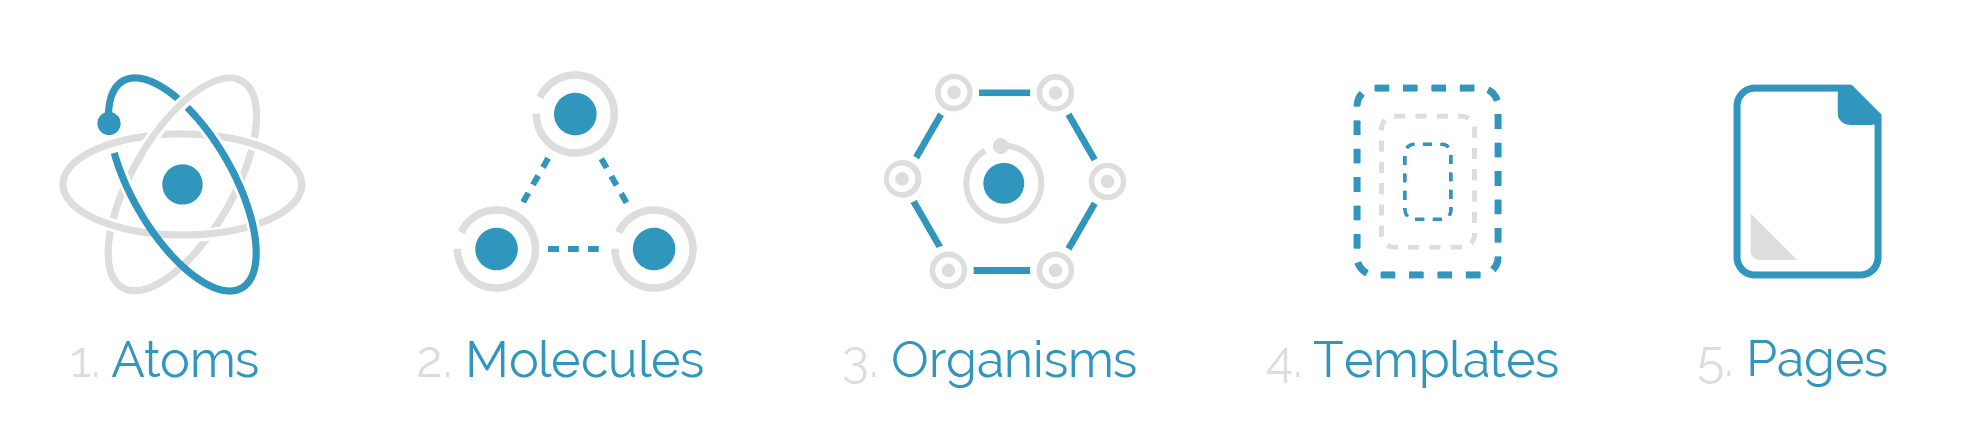
\includegraphics[width=0.8\textwidth]{images/react_atomic_design.png}
	\caption{Diagram \uv{atomického designu} \cite{reactComponentsAtomicDesignDiagram}}
\end{figure}

\section{Lokalizace}
Lokalizace je přizpůsobení textů, formátů dat, měny atd. na stránce (nebo v~aplikaci) tak aby splňovaly jazykové a kulturní požadavky cílené lokality. V~praxi to znamená že v~kódu jsou použity pouze klíče (zkratky) jednotlivých slov, slovních spojení, nebo vět, ke kterým je následně podle souboru s~překlady přiřazena odpovídající hodnota (text). Může být použit jeden soubor s~překlady pro jeden jazyk, nebo být dále rozdělen na několik souborů (např. soubor s~chybovými hláškami, s~vysvětlivkami a ostatní). V~projektu byl vytvořen soubor pro překlad do angličtiny a češtiny. Tyto soubory se nacházejí ve složce \textit{translation/languages}. Jazyk zobrazení je vybrán podle jazyku prohlížeče, pokud se jedná o~nepřihlášeného uživatele, v~opačném případě je nastaven podle uživatelova nastavení. \cite{internationalizationVsLocalization}


\section{Stránka s~mapou}
Stránka s~mapou je výchozí stránka celé webové aplikace (viz obrázek \ref{figure:mapPagePreview}). Pro zobrazení mapy je použit balíček \textit{react-map-gl}, který umožňuje zobrazování např. markerů (značek), polygonů a 3D terénu. Pro zobrazení konkrétních stylů mapy je použit tiling service. Mapa je rozdělena do virtuální mřížky (jedno pole je jeden tzv. tile), pro každý tile je poté ze serveru poslán obrázek korespondující s~konkrétní částí mapy (některé tiling services používají místo rastrové grafiky grafiku vektorovou, což snižuje nároky na síť), server posílá několik tilů zároveň, ty jsou následně cachovány u~klienta. Díky tomu není nutné stahovat data pro jednu část mapy vícekrát. V~projektu byl jako tiling service použit Mapbox, jedná se o~placené řešení s~možností použití již vytvořených stylů, nebo vytvořením stylu zcela vlastního. Alternativou je např. Leaflet, který používá open-source projekt Open street maps. Jeho nevýhodou je malé množství stylů bez možnosti tvorby vlastního.

\begin{figure}[h]
	\centering
	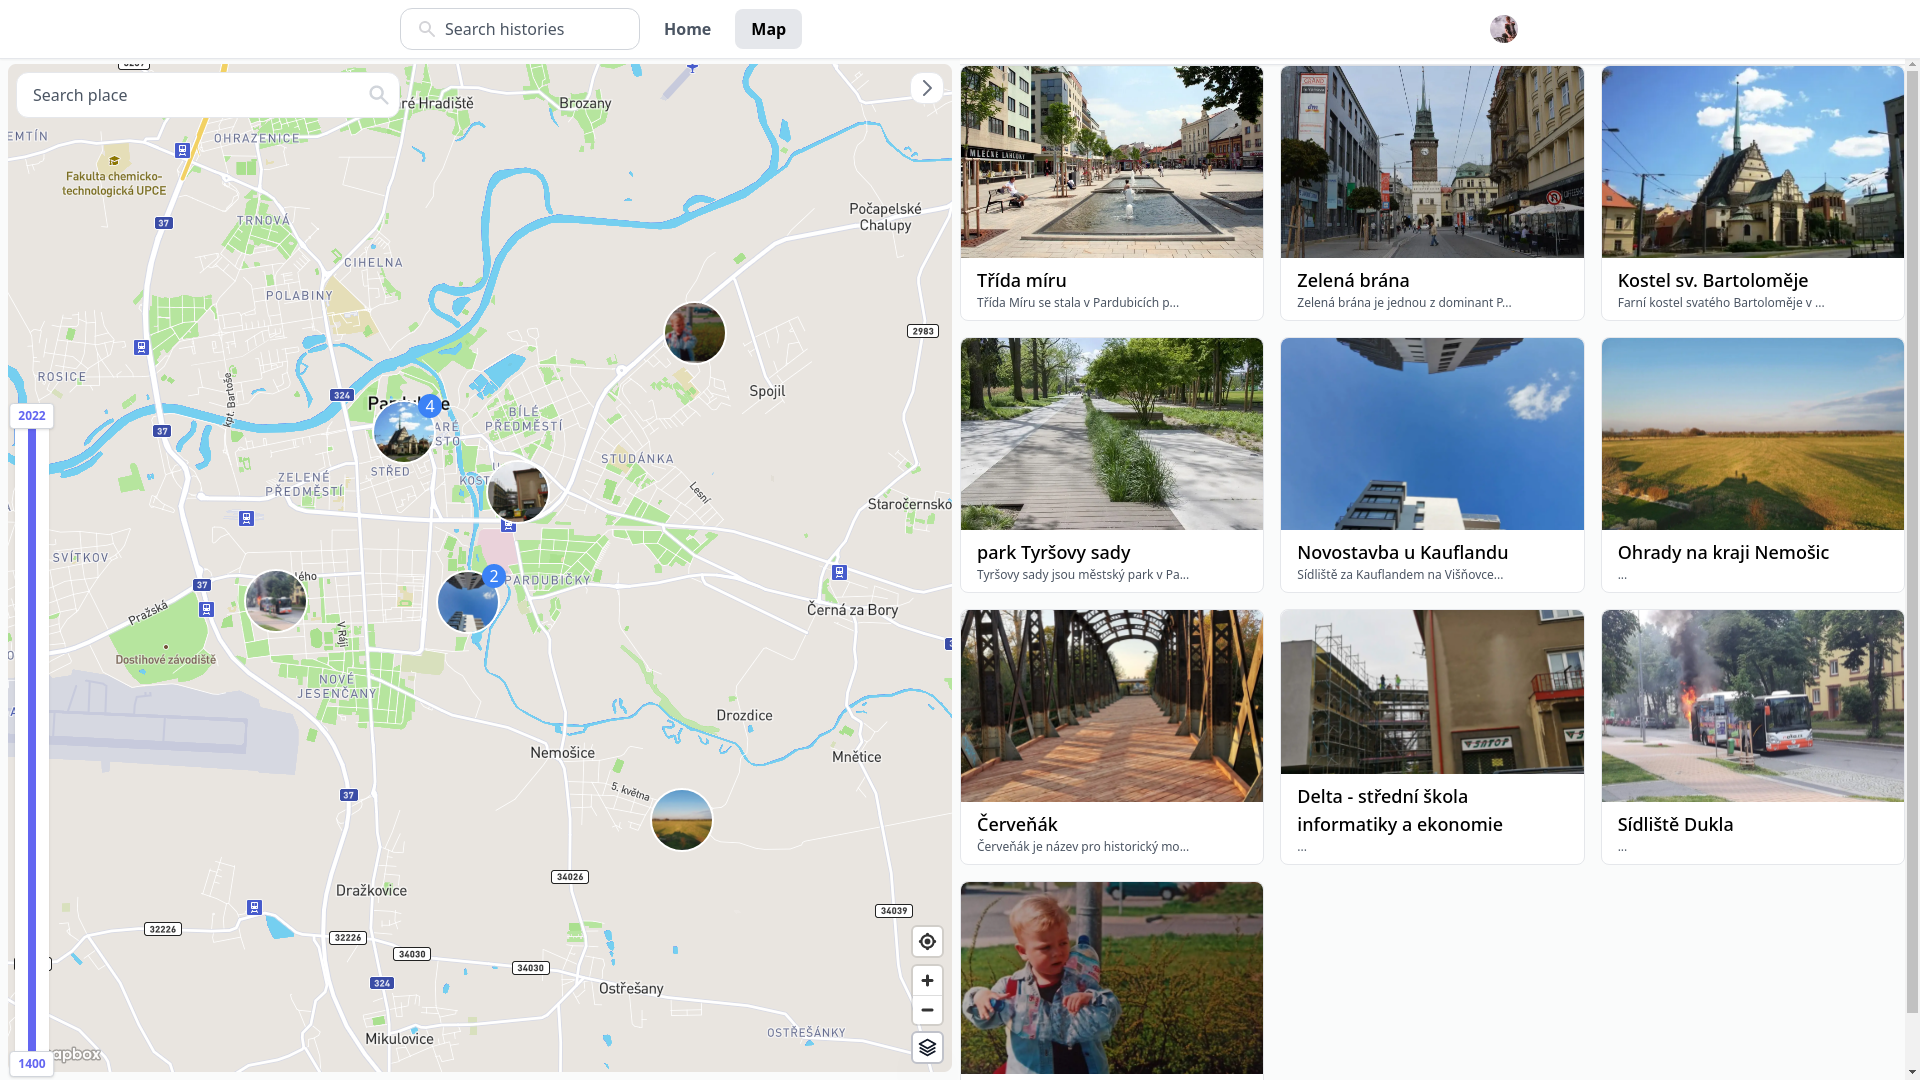
\includegraphics[width=0.8\textwidth]{images/map_page.png}
	\caption{Stránka s~mapou}\label{figure:mapPagePreview}
\end{figure}

\subsection{Zobrazení webové stránky}
Základní zobrazení stránky je rozděleno na pravou a levou část.
\paragraph{Levá část} zobrazuje mapu s~ovládacími prvky. V~levém horním rohu je textový vstup pro vyhledání místa na mapě podle textu. Levý spodní roh obsahuje posuvník znázorňující časovou osu, který umožňuje omezení zobrazených míst a příspěvků podle historického data fotografií, které obsahují. V~pravém spodním rohu jsou tlačítka pro přiblížení a oddálení mapy, přesunutí na aktuální polohu zařázení a menu pro změnu vzhledu mapy. Možné vzhledy mapy jsou světlý, tmavý a satelitní. V~pravém horním rohu se nachází tlačítko umožňující skrýt pravou část a zobrazit mapu přes celou obrazovku.
\paragraph{Pravá část} zobrazuje náhledy všech míst, která se nacházejí v~oblasti mapy a která obsahují příspěvky s~historickým datem odpovídajícím filtrování podle historického data. Toto zobrazení lze přepnout na zobrazení všech příspěvků, které splňují zmíněná kritéria. Při výběru místa se namísto seznamu míst otevře detail vybraného místa obsahující jeho náhled, název, popisek a seznam příspěvků obsahující fotografie daného místa.
\subsection{Geolokace klienta} Pokud parametry URL adresy neobsahují souřadnice na kterých by měla být mapa zobrazena, stránka si vyžádá přístup ke geolokaci. Pokud je přístup udělen, automaticky je lokace mapy nastavena na souřadnice poskytnuté prohlížečem.
\subsection{Ukládání pozice na mapě do parametrů URL adresy}
Při každém pohybu po mapě jsou souřadnice aktuální pozice mapy uloženy do paramterů URL adresy. Díky tomu při obnovení stránky pozice mapy zůstává nezměněna. Tato funkcionalita byla inspirována např. Mapy.cz a Google maps. Toto také umožňuje uživateli sdílet aktuální zobrazení mapy zkopírováním URL adresy.
\subsection{Načítání míst na mapě}
Vzhledem k~tomu že množství míst na mapě není teoreticky nijak omezeno, musí být načítána postupně. Pokud by ale byla načítána nová místa při každém pohybu, nebyl by pohyb po mapě plynulý a z~toho důvodu téměř nepoužitelná (kvůli množství dotazů na API). Tento problém byl vyřešen tím, že dotaz na API je odeslán po dokončení pohybu. Pro zmenšení objemu přenesených dat každý takový požadavek obsahuje seznam míst, která byla již dříve načtena a nacházejí se v~zobrazené oblasti, tato místa jsou vynechána z~odpovědi serveru.
\clearpage
\subsection{Zobrazení míst na mapě}
Místo na mapě je zobrazeno jako fotografie v~kruhu, nacházející se na souřadnicích daného místa viz obrázek \ref{figure:onePlaceOnMap}. Pro optimalizaci mapy jsou vykreslovány pouze místa nacházející se v~zobrazené oblasti.
\subsection{Seskupování míst na mapě}
Při oddálení mapy by se v~případě většího počtu zobrazených míst mohla daná místa překrývat, snižovat přehlednost mapy a zpomalovat pohyb po mapě. Z~toho důvodu je použit tzv. clustering (shlukování více bodů), místo těchto bodů je následně vykreslen pouze jeden, který se nachází na souřadnicích průměru souřadnic všech bodů, které cluster obsahuje viz obrázek \ref{figure:clusterOnMap}. Pro rozhodnutí, který obrázek bude na mapě zvolen jako náhled clusteru jsou porovnány vzdálenosti všech míst, která cluster obsahuje od středu clusteru. jako náhled je použit náhled místa, které je nejblíže středu clusteru. V~pravém vrchním rohu náhledu je poté zobrazeno číslo vyjadřující počet míst seskupených v~clusteru. Při kliknutí na náhled clusteru je mapa přiblížena tak aby bylo zobrazeno co nejvíce míst jako samostatná místa a ne clustery.

\begin{figure}[!h]

	\centering
	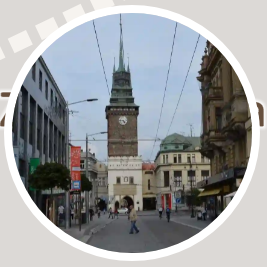
\includegraphics[width=4cm]{images/place.png}
	\caption{Zobrazení jednoho místa na mapě}\label{figure:onePlaceOnMap}
	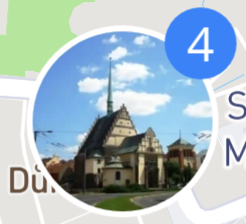
\includegraphics[width=4cm]{images/places_cluster.png}
	\caption{Zobrazení seskupení několika míst na mapě}\label{figure:clusterOnMap}

\end{figure}



\section{Stránka domů}
Pro lepší představu je tato stránka ukázána na obrázku \ref{figure:homePagePreview}. Stránka domů slouží k~prohlížení nových příspěvků od uživatelů, které uživatel sleduje. Zároveň obsahuje sekci doporučení uživatelé a zajímavá místa, které uživateli umožňují objevovat nové uživatele a místa. Pokud uživatel není přihlášen, jsou zde zobazeni nejpopulárnější uživatelé a nejoblíbenější příspěvky. Pro nejlepší UX (user experience) je použit infinite scroll (nekonečné rolování), které zajišťuje dostatek obsahu a průběžné načítání dalších příspěvků, které mají být zobrazeny.

\begin{figure}[h]
	\centering
	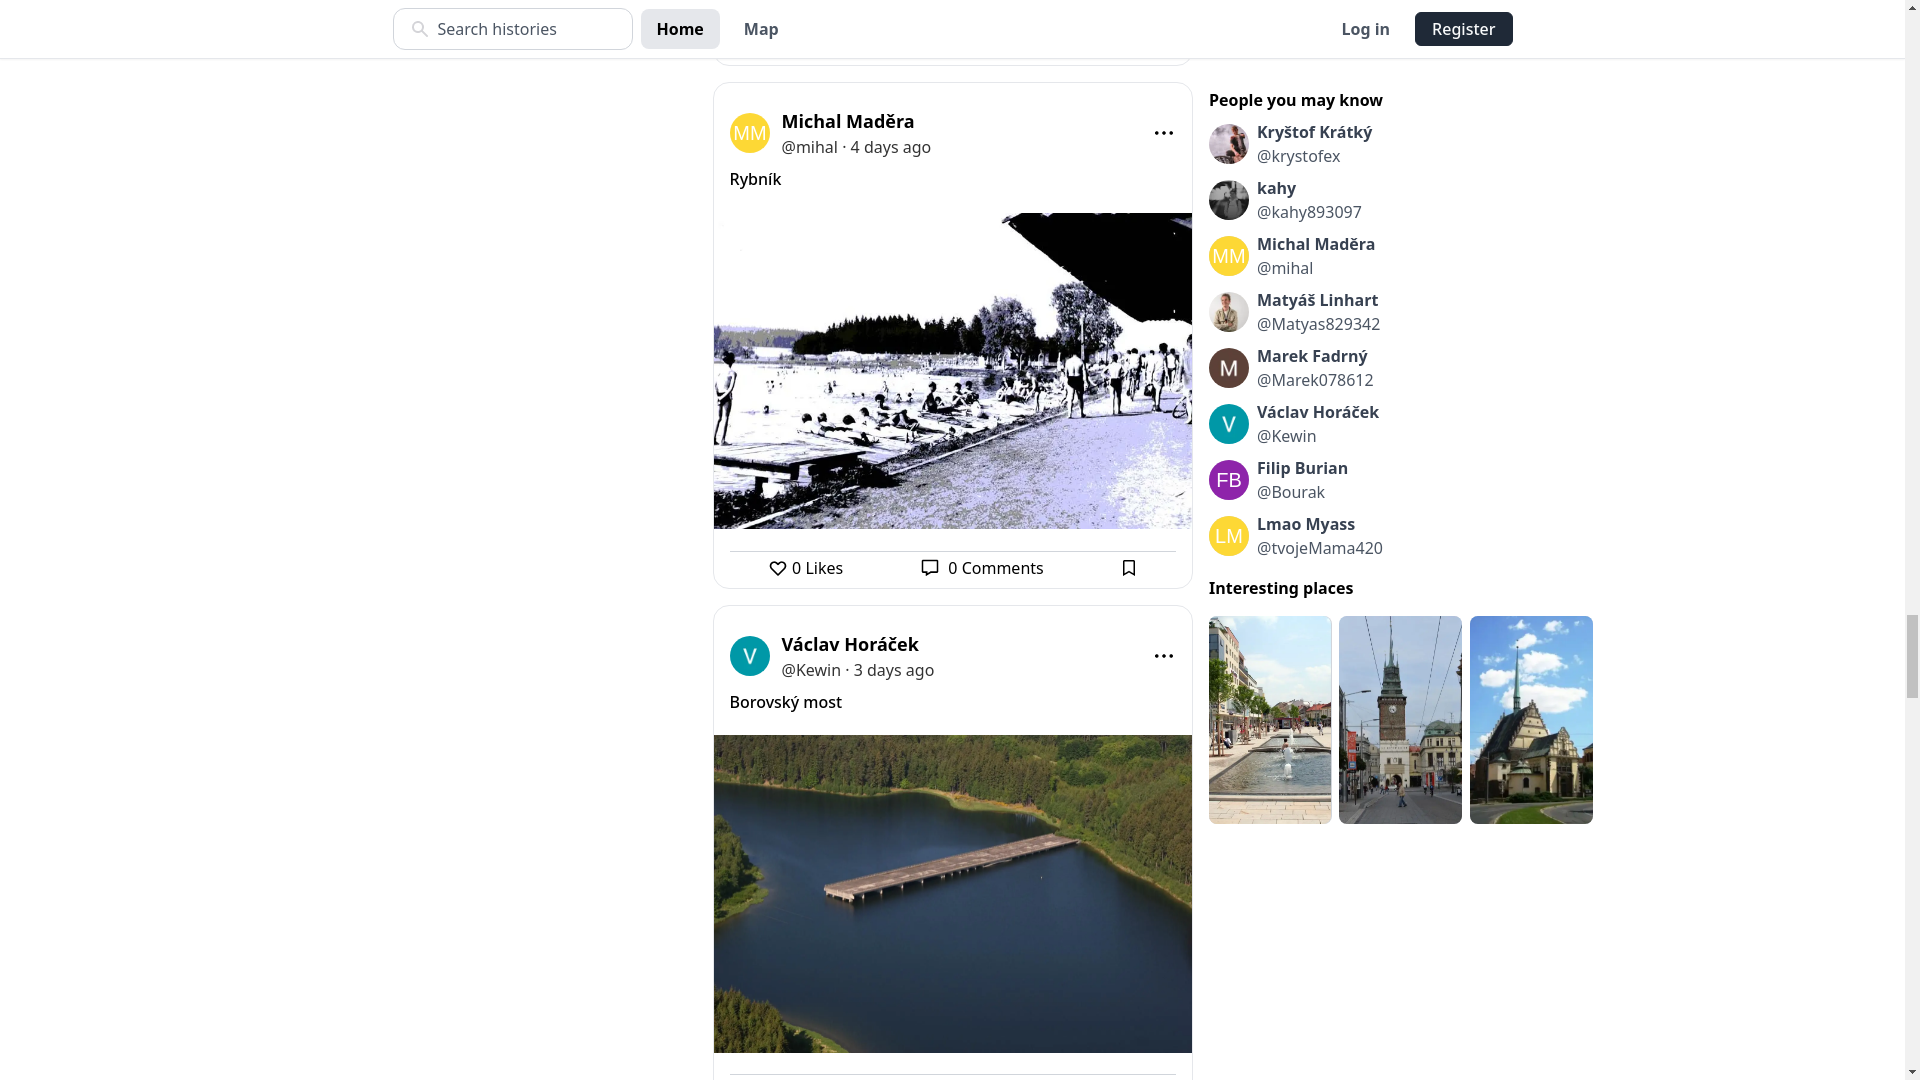
\includegraphics[width=0.8\textwidth]{images/home_page.png}
	\caption{Domovská stránka}\label{figure:homePagePreview}
\end{figure}

\section{Komentáře}
Komentáře umožňují uživateli reagovat na příspěvky a komentáře ostatních uživatelů, nebo s~nimi vést diskuze. Hloubkou komentářového vlákna je označováno maximální možné množství na sebe do sebe zanořených komentářů. V~projektu je omezena na jednu úroveň (lze komentovat příspěvky a komentáře příspěvků) kvůli větší přehlednosti a intuitivnějšímu ovládání. Komentáře jsou velice důležité pro vyjadřování názorů a zapojení nových uživatelů do komunity. Zároveň jsou komentáře užitečné např. při vyhodnocování popularity příspěvků, nebo analýze komunity pomocí sociálního grafu.
\cite{whyAreCommentsImportant}

\section{Profilová stránka uživatele}
Profilová stránka zobrazuje všechny informace o~uživateli (viz obrázek \ref{profilePageScreenshot}). Tato stránka se nachází na URL adrese závislé na uživatelském jménu, např. profilová stránka uživatele s~uživatelským jménem \uv{Joe} by se nacházela na adrese \textit{/user/joe} (nerozlišují se velká a malá písmena v~uživatelském jméně). Hlavní rozložení stránky je rozděleno na levý panel zabírající přibližně čtvrtinu obrazovky a hlavní obsah zabírající zbytek obrazovky. Ve vrchní části hlavního obsahu je navigační lišta, ve které je možné přepínat mezi třemi záložkami, podle kterých se mění obsah zobrazený v~hlavní části.
\clearpage
\subsection{Levý panel}
Levý panel zobrazuje veškeré informace o~daném uživateli. Ve vrchní části je zobrazena uživatelova profilová fotografie. Pod profilovou fotografií je uživatelovo jméno a příjmení. Dále je zde uživatelské jméno, vedle kterého se zobrazují tzv. bannery. Mezi možné bannery patří např. \uv{ověřený uživatel} (viz \ref{paragraph:verifiedUser}), \uv{nový uživatel} (je zobrazen po dobu tří dnů od založení účtu), nebo \uv{admin} (viz \ref{paragraph:usersWithAdminPermissions})

\begin{figure}[h]
	\centering
	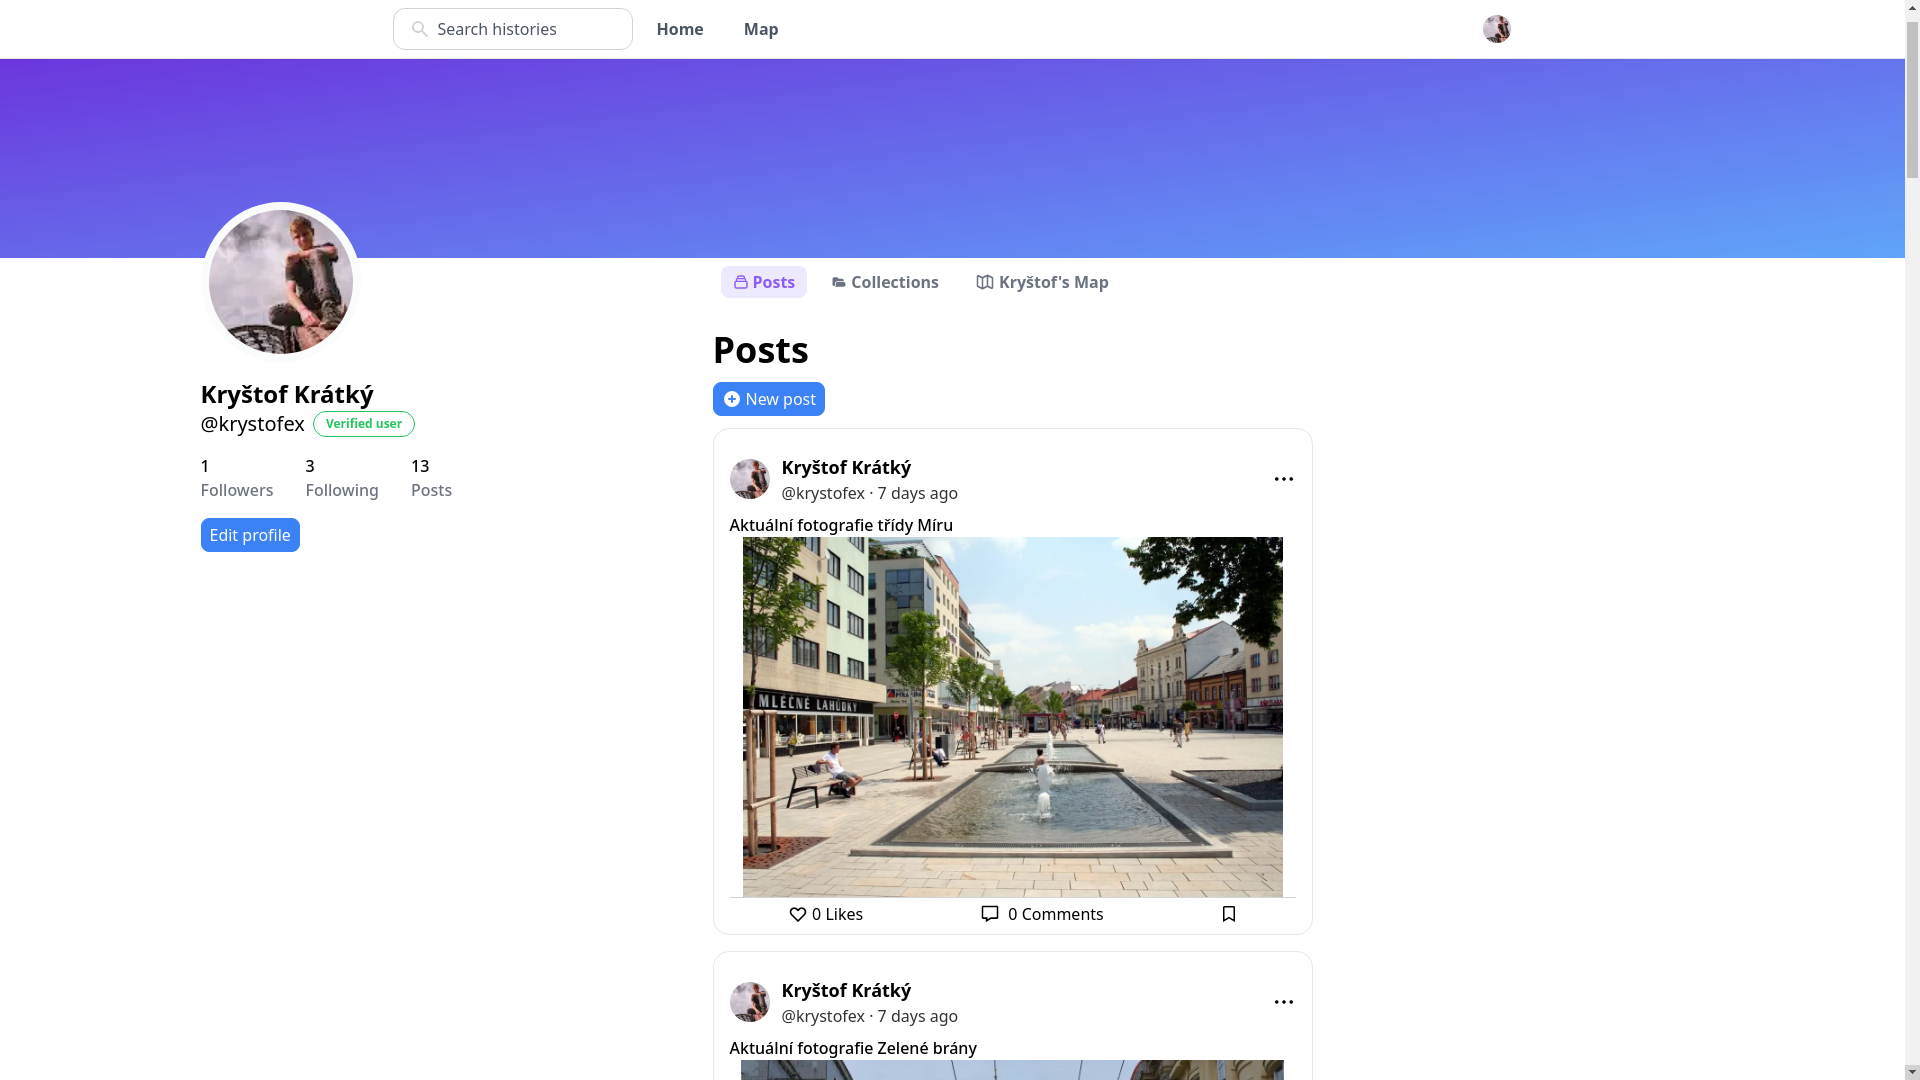
\includegraphics[width=0.8\textwidth]{images/user_page.png}
	\caption{Profilová stránka uživatele}\label{profilePageScreenshot}
\end{figure}

\subsection{Záložka příspěvky}
Jednu se o~nejdůležitější záložku. Na této záložce jsou zobrazeny všechny příspěvky, které uživatel vytvořil seřazeny od nejnovějšího po nejstarší. Každý příspěvek je zobrazen v~kartě. Karta se skládá ze tří hlavních částí: vrchní panel, fotografie a spodní panel. 
\subsubsection{Vrchní panel}
V~levé vrchní části vrchního panelu jsou informace o~autorovi příspěvku, jako je jeho jméno, uživatelské jméno a profilová fotografie. Vedle uživatelského jména je zobrazeno, před jak dlouhou dobou byl příspěvek vytvořen. Pod těmito informacemi se nachází uživatelův popisek. V~pravém části vrchního panelu je tlačítko pro zobrazení více možností. Po kliknutí na tlačítko více možností se otevře menu obsahující různé možnosti podle typu uživatele.
\begin{itemize}
    \item \textbf{Nepřihlášení uživatelé} vidí možnosti \uv{zobrazit detail příspěvku} a \uv{zkopírovat odkaz na příspěvek}
    \item \textbf{Přihlášení uživatelé}, kteří zároveň nejsou autorem příspěvku vidí kromě stejných možností, jako uživatelé nepřihlášení také možnost příspěvek nahlásit.
    \item \textbf{Autor příspěvku} vidí kromě stejných možností jako nepřihlášení uživatelé také možnosti \uv{smazat příspěvek} a \uv{upravit příspěvek}
    \item \textbf{Administrátor} administrátor vidí stejné možnosti jako autor příspěvku rozšířené o~možnost \uv{označit příspěvek jako NSFW}, případně \uv{odznačit příspěvek jako NSFW}
\end{itemize}
\subsubsection{Fotografie}
Pod vrchním panelem se nachází část s~fotografií. Pokud příspěvek obsahuje více fotografií, je možné se mezi nimi přesouvat pomocí šipek na levé a pravé straně. Při kliknutí na fotografii je otevřeno dialogové okno, které umožňuje si fotografii detailněji prohlédnout. 
\subsubsection{Spodní panel}
V~levé části spodního panelu je tlačítko \textit{to se mi líbí}. Pokud je uživatel přihlášen, může označit příspěvek jako to se mi líbí. U~takto označeného příspěvku je tlačítko vyplněno červenou barvou, v~opačném případě je tlačítko zobrazeno pouze jako obrys. Vedle tohoto tlačítka je zobrazen celkový počet uživatelů, kteří tento příspěvek označili jako to se mi líbí. V~prostřední části spodního panelu je zobrazena ikona komentáře společně s~celkovým počtem komentářů k~příspěvku. Po kliknutí na ikonu komentáře je uživatel přesměrován na detail příspěvku, kde je možné zobrazit jednotlivé komentáře, nebo napsat vlastní komentář. V~pravé části spodního panelu se nachází ikona záložky. Po kliknutí na ikonu záložky je otevřeno dialogové okno, ve kterém je možné přidat příspěvek do jakékoliv z~kolekcí přihlášeného uživatele.
\subsection{Záložka kolekce}
Na této stránce jsou zobrazeny všechny uživatelovy kolekce, ke kterým má přístup aktuální uživatel (pokud má přihlášený uživatel administrátorská oprávnění, jsou zobrazeny všechny kolekce, jinak jsou zobrazeny pouze veřejné kolekce). Kolekce je znázorněna jako karta, na které je název kolekce, její popis a počet příspěvků, které kolekce obsahuje. Po kliknutí na kolekce je zobrazen detail kolekce, ve kterém jsou zobrazeny všechny příspěvky zarovnané do mřížky. Při kliknutí na jakýkoliv příspěvek je otevřen jeho detail, ve kterém je možné zobrazit předchozí, nebo následující příspěvek v~kolekci. Ve vrchní části kolekce je také možnost příspěvky seřadit. Možnosti řazení jsou: od nejoblíbenějšího, od nejstaršího podle historického data, od nejnovějšího podle historického data, od nejstaršího podle času vytvoření, a od nejnovějšího, nebo nejnovějšího podle času vytvoření. Pokud je přihlášený uživatel autor kolekce, má možnost upravit jméno a popis kolekce, nebo kolekci smazat.
\subsection{Záložka uživatelova mapa}
Na této mapě jsou označena všechna místa, ke kterým uživatel přidal příspěvek. Tato mapa slouží čistě pro shrnutí a nemá nahrazovat hlavní mapu. Proto zde nejsou zobrazeny žádné fotografie ani možnost jakékoliv jiné interakce než prohlížení mapy.

\section{Stránka detail příspěvku}
Rozložení stránky je rozděleno na pravou a levou část. Hlavním účelem levé části je zobrazení fotografií příspěvku. Nad fotografií je zobrazena ikona kalendáře společně s~historickým datem. Po kliknutí na ikonu kalendáře bude uživatel přesměrován na mapu, kde je automaticky nastaveno filtrování. Pokud má příspěvek nastaveno přesné datum, omezí filtr na zobrazení všech příspěvky v~rozsahu mezi 20 lety před datem příspěvku a 20 lety po datu příspěvku. Pokud je datum příspěvku stanoveno v~rozmezí několika let, je filtrování nastaveno podle tohoto rozmezí. Hlavní část zabírá fotografie místa, pod kterou je tlačítko líbí se mi a pokud má příspěvek více fotografií možnost mezi nimi posouvat. V~pravé části se nachází komentářová sekce.


\chapter{Vývoj}
\section{Nasazení na server}
\subsection{Docker}
Docker je soubor platforem a služeb poskytujících virtualizaci na úrovni operačního systému pro spouštění softwaru v~balíčcích nazývané kontejnery. Docker zajišťuje že programy a aplikace vždy poběží ve stejném prostředí nezávisle na zařízení nebo operačním systému. Jednoduchost spuštění kontejneru usnadňuje nasazení aplikace na server. Celý projekt včetně databáze a úložiště je pak možné spustit jedním skriptem bez nutnosti nastavování.
\subsection{Hosting}
Jako hosting je označována služba, na kterou lze nahrát svou webovou aplikaci, která následně bude přístupná na internetu. Pro hostování aplikace byla zvolena platforma DigitalOcean, z~důvodu jednoduchosti administrátorského rozhraní (na rozdíl od např. AWS) a ceně. Zároveň nabízí funkce jako například automatické naklonování aplikace z~Git repozitáře a následné spuštění na serveru při změně kódu. Umožňuje také pronajmutí virtuálního počítače, na kterém lze následně aplikaci spustit například v~Docker kontejneru.

\section{Verzování}
Git je software pro sledování změn v~souborech, které jsou součástí repozitáře. Git poskytuje možnost se kdykoliv vrátit do jakékoliv verze projektu. Git lze také použít při kolaboraci více programátorů, nebo pro synchronizaci kódu.
\section{Testování}
\subsection{Při vývoji}
\paragraph{Unit testing} je automatizované testování jednotlivých funkcí kódu zadáním vstupních parametrů a následným porovnání výsledků s~očekávanými výsledky.
\paragraph{Linter} je označení pro skupinu nástrojů, analyzující statický kód bez nutnosti jeho spuštění. Zároveň zajišťuje jednostnost kódu kontrolou pravidel pro formátování.


\chapter{Závěr}
V~rámci projektu se podařilo vyvinout webovou aplikaci umožňující uživatelům sdílet a prohlížet historické fotografie. V~současné době má uživatel možnost vytvářet vlastní příspěvky, prohlížet příspěvky ostatních uživatelů, ukládat příspěvky do kolekcí a interagovat s~ostatními uživateli pomocí komentářů. Veškerý nahraný obsah prochází kontrolou proti nevhodnému obsahu. Aplikace je zcela připravena pro použití reálnou komunitou, na základě jejíž zpětné vazby bude moci být dále vyvíjena a upravována.

%% obrázky 
\listoffigures

%% Citace
\begin{thebibliography}{100}

    \bibitem{NSFW} NSFW Meaning, what does NSFW mean in text \textit{myenglishteacher.eu} [online]. [cit. 2022-03-19]. Dostupné z: \url{https://www.myenglishteacher.eu/blog/nsfw-meaning/}
    
    \bibitem{GarbageCollection} The Very Basics of Garbage Collection \textit{basen\.oru\.se} [online]. [cit. 2022-03-19]. Dostupné z: \url{http://basen.oru.se/kurser/koi/2008-2009-p1/texter/gc/index.html/}
    
    \bibitem{whatIsRuntimeEnvironment} What Does Runtime Environment (RTE) Mean \textit{Techopedia} [online]. [cit. 2022-03-19]. Dostupné z: \\ \url{https://www.techopedia.com/definition/5466/runtime-environment-rte}
    
    \bibitem{PardubiceVBehuCasuFB} Zajímavosti, videa a obrázky z historie Pardubic \textit{Pardubice v běhu času} [online]. [cit. 2022-03-19]. Dostupné z: \url{https://www.facebook.com/groups/starepardubice/}
    
    \bibitem{DynamicVsStaticTyping} Dynamic typing vs. static typing \textit{Oracle docs} [online]. [cit. 2022-03-19]. Dostupné z: \\ \url{https://docs.oracle.com/cd/E57471_01/bigData.100/extensions_bdd/src/cext_transform_typing.html}
    
    \bibitem{whatIsTypescript} What is typescript \textit{typescripttutorial.net} [online]. [cit. 2022-03-19]. Dostupné z: \url{https://www.typescripttutorial.net/typescript-tutorial/what-is-typescript/}
    
    \bibitem{typescriptForTheNewProgrammer} TypeScript for the New Programmer \textit{Typescript docs} [online]. [cit. 2022-03-19]. Dostupné z: \url{https://www.typescriptlang.org/docs/handbook/typescript-from-scratch.html/}
    
    \bibitem{whatIsNpmW3} What is npm \textit{W3 schools} [online]. [cit. 2022-03-19]. Dostupné z: \url{https://www.w3schools.com/whatis/whatis_npm.asp}
    
    \bibitem{aboutNpm} About npm \textit{NPM docs} [online]. [cit. 2022-03-19]. Dostupné z: \url{https://docs.npmjs.com/about-npm}
    
    \bibitem{graphqlIntroduction} Introduction to GraphQL \textit{GraphQL} [online]. [cit. 2022-03-19]. Dostupné z: \url{https://graphql.org/learn/}
    
    \bibitem{graphqlTypes} Schemas and Types \textit{GraphQL} [online]. [cit. 2022-03-19]. Dostupné z: \url{https://graphql.org/learn/schema/#type-system}
    
    \bibitem{restApiRedHat} What is REST API? \textit{Red Hat} [online]. [cit. 2022-03-19]. Dostupné z: \url{https://www.redhat.com/en/topics/api/what-is-a-rest-api/}
    
    \bibitem{whatIsApiAws} What is an API? \textit{Amazon AWS} [online]. [cit. 2022-03-19]. Dostupné z: \url{https://aws.amazon.com/what-is/api/}
    
    \bibitem{whatIsFrontend} Frontend vs. backend: what's the difference? \textit{Pluralsight} [online]. [cit. 2022-03-19]. Dostupné z: \url{https://www.pluralsight.com/blog/software-development/front-end-vs-back-end/T}
    
    \bibitem{reactComponentsAndProps} Components and Props \textit{React docs} [online]. [cit. 2022-03-19]. Dostupné z: \url{https://reactjs.org/docs/components-and-props.html}
    
    \bibitem{gettingStartedReact} Getting started \textit{React docs} [online]. [cit. 2022-03-19]. Dostupné z: \url{https://reactjs.org/docs/getting-started.html}
    
    \bibitem{whatIsSSR} Client-side vs. server-side rendering \textit{Free code camp} [online]. [cit. 2022-03-19]. Dostupné z: \url{https://www.freecodecamp.org/news/what-exactly-is-client-side-rendering-and-hows-it-different-from-server-side-rendering-bd5c786b340d/}
    
    \bibitem{whatIsSEO} What Is SEO \textit{Next.js docs} [online]. [cit. 2022-03-19]. Dostupné z: \url{https://moz.com/learn/seo/what-is-seo}
    
    \bibitem{nextGetStarted} Gettings started \textit{Next.js docs} [online]. [cit. 2022-03-19]. Dostupné z: \url{https://nextjs.org/docs/getting-started}
    
    \bibitem{tailwindDocumentation} Get started with Tailwind CSS \textit{Tailwind CSS} [online]. [cit. 2022-03-19]. Dostupné z: \url{https://tailwindcss.com/docs/installation/}
    
    \bibitem{graphqlCodeGeneratorDocs} Introduction to GraphQL Code Generator \textit{GraphQL code generator docs} [online]. [cit. 2022-03-19]. Dostupné z: \url{https://www.graphql-code-generator.com/docs/getting-started}
    
    \bibitem{aboutNodeJS} About Node.js® \textit{Node.js®} [online]. [cit. 2022-03-19]. Dostupné z: \url{https://nodejs.org/en/about/}
    
    \bibitem{IPFSDocs} IPFS is a distributed system for storing and accessing files, websites, applications, and data \textit{IPFS} [online]. [cit. 2022-03-19]. Dostupné z: \url{https://docs.ipfs.io/}
    
    \bibitem{decentralizedVsTrustless} Decentralized vs Trustless Networks \textit{Bluzelle} [online]. [cit. 2022-03-19]. Dostupné z: \url{https://bluzelle.com/blog/decentralized-vs-trustless-networks}
    
    \bibitem{decentralizedAndDistributedNetworks} Centralized, Decentralized, \& Distributed Networks \textit{Cryptopedia} [online]. [cit. 2022-03-19]. Dostupné z: \url{https://www.gemini.com/cryptopedia/blockchain-network-decentralized-distributed-centralized}
    
    \bibitem{decentralizedAndTrustless} Decentralized and Trustless Networks \textit{Hackernoon} [online]. [cit. 2022-03-19]. Dostupné z: \url{https://hackernoon.com/decentralized-and-trustless-networks-f881671fae4e}
    
    \bibitem{IPFScontentAddressing} Content addressing and CIDs \textit{IPFS} [online]. [cit. 2022-03-19]. Dostupné z: \url{https://docs.ipfs.io/concepts/content-addressing/}
    
    \bibitem{IPFSPersistence} Persistence | IPFS Docs \textit{IPFS} [online]. [cit. 2022-03-19]. Dostupné z: \url{https://docs.ipfs.io/concepts/persistence/}
    
    \bibitem{IPFSgateways} IPFS Gateway \textit{IPFS} [online]. [cit. 2022-03-19]. Dostupné z: \url{https://docs.ipfs.io/concepts/ipfs-gateway/}
    
    \bibitem{whatIsS3} What is Amazon S3? \textit{Amazon AWS} [online]. [cit. 2022-03-19]. Dostupné z: \url{https://docs.aws.amazon.com/AmazonS3/latest/userguide/Welcome.html}
    
    \bibitem{whatIsDatabase} What Is a Database? \textit{Oracle} [online]. [cit. 2022-03-19]. Dostupné z: \url{https://www.oracle.com/database/what-is-database/}
    
    \bibitem{whatIsACID} The ACID Database Model \textit{Lifewire} [online]. [cit. 2022-03-19]. Dostupné z: \url{https://www.lifewire.com/the-acid-model-1019731/}
    
    \bibitem{graphenTheorie} Graphentheorie \textit{Mathepedia} [online]. [cit. 2022-03-19]. Dostupné z: \url{https://mathepedia.de/Graphentheorie.html}
    
    \bibitem{graphDatabasesIntroduction} Graph Databases for Beginners: Why Graph Technology Is the Future \textit{Neo4j} [online]. [cit. 2022-03-19]. Dostupné z: \url{https://neo4j.com/blog/why-graph-databases-are-the-future/}
    
    \bibitem{graphAlgorithms} Graph Algorithms in Neo4j: Neo4j Graph Analytics \textit{Neo4j} [online]. [cit. 2022-03-19]. Dostupné z: \url{https://neo4j.com/blog/graph-algorithms-in-neo4j-neo4j-graph-analytics/}
    
    \bibitem{aboutNeo4j} The Fastest Path to Graph \textit{Neo4j} [online]. [cit. 2022-03-19]. Dostupné z: \url{https://neo4j.com}
    
    \bibitem{CypherQL} Cypher Query Language \textit{Neo4j} [online]. [cit. 2022-03-19]. Dostupné z: \url{https://neo4j.com/developer/cypher/}
    
    \bibitem{Neo4jNamingRules} Naming rules and recommendations - Neo4j Cypher Manual \textit{Neo4j} [online]. [cit. 2022-03-19]. Dostupné z: \url{https://neo4j.com/docs/cypher-manual/4.4/syntax/naming/}
    
    \bibitem{Neo4jSparialFunctions} Spatial functions - Neo4j Cypher Manual \textit{Neo4j} [online]. [cit. 2022-03-19]. Dostupné z: \url{https://neo4j.com/docs/cypher-manual/4.4/functions/spatial/}
    
    \bibitem{nextImage} API documentation for the Image Component and Image Optimization \textit{Next.js docs} [online]. [cit. 2022-03-19]. Dostupné z: \url{https://nextjs.org/docs/api-reference/next/image}
    
    \bibitem{blurhash} BlurHash is a compact representation of a placeholder for an image \textit{Blurhash} [online]. [cit. 2022-03-19]. Dostupné z: \url{https://blurha.sh/}
    
    \bibitem{blurhashWoltBlog} How we came to create a new image placeholder algorithm, BlurHash \textit{Wolt blog} [online]. [cit. 2022-03-19]. Dostupné z: \url{https://blog.wolt.com/hq/2019/07/01/how-we-came-to-create-a-new-image-placeholder-algorithm-blurhash/}
    
    \bibitem{blurhashScreenshot} Obrázek převzat z https://blurha.sh \textit{Blurhash} [online]. [cit. 2022-03-19]. Dostupné z: \url{https://blurha.sh/}
    
    \bibitem{reactComponentsAtomicDesign} Atomic Design Methodology \textit{bradfrost.com} [online]. [cit. 2022-03-19]. Dostupné z: \url{https://atomicdesign.bradfrost.com/chapter-2/}
    
    \bibitem{reactComponentsAtomicDesignDiagram} Diagram atomického designu \textit{Github} [online]. [cit. 2022-03-19]. Dostupné z: \url{https://user-images.githubusercontent.com/4838076/33235048-d083dca6-d217-11e7-9aea-9a5ef5ae6fe7.png}
    
    \bibitem{internationalizationVsLocalization} Internationalization vs. localization (i18n vs l10n): What’s the difference? \textit{Lokalise} [online]. [cit. 2022-03-19]. Dostupné z: \url{https://lokalise.com/blog/internationalization-vs-localization/}
    
    \bibitem{whyAreCommentsImportant} Reasons Why Comments Are Important For Instagram \textit{Time square chronicles} [online]. [cit. 2022-03-19]. Dostupné z: \url{https://t2conline.com/reasons-why-comments-are-important-for-instagram/}
    
    
    \bibitem{bootstrap} Build fast, responsive sites with Bootstrap \textit{Bootstrap} [online]. [cit. 2022-03-19]. Dostupné z: \url{https://getbootstrap.com/}
    
    
    \end{thebibliography}
    
    %%%%% CLEAR DOUBLE PAGE!
    \newpage{\pagestyle{empty}\cleardoublepage}


\end{document}
